\documentclass[conference]{IEEEtran}
\usepackage[T1]{fontenc}
\usepackage{amsmath,amssymb,amsfonts}
\usepackage{bm}
\usepackage{booktabs}
\usepackage{graphicx}
\usepackage{cite}
\usepackage{url}
\usepackage{algorithm}
\usepackage{algorithmic}

\newcommand{\KVTTT}{\textsc{KV-TTT}}
\newcommand{\kernel}[1]{\bm{Z}^{(#1)}}

\begin{document}

\title{Post-Visual Residual Key--Value Test-Time Tuning for Event-Adaptive Remote-Sensing Damage Assessment}

\author{\IEEEauthorblockN{Anonymous Author}
\IEEEauthorblockA{\textit{Anonymous institution, submitted to ICASSP 2027}}}

\maketitle

\begin{abstract}
Building-damage assessment from paired pre-/post-event satellite imagery is high-stakes, yet every newly unfolding disaster is an implicit distribution shift for any fixed model. We propose Post-Visual Residual \emph{Key--Value Test-Time Tuning} (\KVTTT{}), a weight-disjoint, budget-bounded adaptation that operates exclusively in the activations of a frozen source VLM. Given a tiny balanced support set collected after the event, \KVTTT{} (1) back-propagates a label-token loss through a frozen decoder and collects ``correctness gradients'' on the \emph{post-event} image tokens for a few $k$/$v$-projection outputs; (2) assembles their covariance into a low-rank corrective subspace $\bm{B}$; (3) injects a masked, bounded residual $\bm{Z}'=\bm{Z}+\bm{M}\odot\big((\bm{Z}\bm{B})\,\mathrm{diag}(\alpha_{\max}\tanh \bm{a})\,\bm{B}^{\top}\big)$ on those rows; and (4) fits the 64 bounded scalars $\bm{a}$ with four full-batch Adam steps over the support. We report leave-one-event-out results on \textsc{BRIGHT} ($244{,}976$ instances): across the completed folds \KVTTT{} improves macro-F1 and calibration on the large majority (5/6 folds now; the full $11$-event protocol is queued), is stable across three source seeds, and beats the weight-space baseline that fine-tunes the same twelve support instances into the LoRA (which overfits and collapses the model). A cross-event variant that reuses a subspace from other disasters performs on par with the online one. No weight is touched; only the residual is moved.
\end{abstract}

\begin{IEEEkeywords}
test-time adaptation, building damage assessment, remote sensing, vision--language models, key--value memory.
\end{IEEEkeywords}

\section{Introduction}
\IEEEPARstart{B}{uilding}-damage assessment is one of the first and most decision-relevant signals available after a disaster: for every building footprint in a populated area the analyst needs to know whether it is \emph{intact}, \emph{damaged} or \emph{destroyed}, using a pre-event reference and a freshly acquired post-event image. Automating it matters precisely because the surveying institutions themselves are often incapacitated at the moment the answer is needed.

Vision--language models (VLMs) are strong candidates: they carry rich visual priors~\cite{radford2021clip}, produce calibrated per-class scores, and adapt well to remote sensing via low-rank fine-tuning~\cite{hu2021lora,qwen2_5vl}. Yet every new disaster event is a distribution shift in disguise --- different sensor, geometry, lighting, land cover, and damage semantics. A model that performs well on source data degrades, sometimes abruptly, on the event it is deployed to first. The conventional remedy---weight fine-tuning even at low rank---is brittle when the adaptation budget is a dozen samples: it memorizes the support and collapses confidence. In our measurements, updating the source LoRA on exactly the twelve support examples that \KVTTT{} also sees drives macro-F1 on the target from $0.387$ to $0.171$ and NLL from $3.4$ to $14.6$.

We take a different route. A transformer is a deep key--value architecture~\cite{vaswani2017attention}: each decoder layer projects its context into keys and values that feed attention~\cite{geva2021kv,brown2020gpt3}. The \emph{weights} encode the general prior; the \emph{activations} of the $k$/$v$ projections carry instance-specific evidence about the post-event change. Our key observation is that, at support time, the label-token loss induces a concentrated, low-rank gradient exactly on the post-event image-token rows of those projections. We collect these ``correctness gradients'', summarize them into a low-rank subspace $\bm{B}$, and fit a handful of bounded scalar gates that reshape only those token rows in $k$/$v$ output space. The model, its LoRA, its text tokens, and its pre-event image tokens never change. The result is adaptation that is weight-disjoint, bounded between identity and a maximal gate (at zero coefficients the frozen model is bit-exact), deterministic (full-batch, no sampling), and cheap (one forward pass per query at inference). Figure~\ref{fig:per} and Table~\ref{tab:main} report leave-one-event-out isolation on \textsc{BRIGHT}~\cite{bright2024}.

\section{Related Work}
\textbf{Test-time adaptation.} Test-time training~\cite{sun2020ttt}, TENT~\cite{wang2020tent}, and their online/continual extensions~\cite{wang2022cotta} modify normalization statistics or the training objective at inference, usually assuming an unlabelled test stream and changing per-sample feature statistics. For VLMs, test-time prompt tuning~\cite{shu2022tpt} optimizes a soft prompt on unlabelled test batches; this needs a batch of correlated samples and still changes a weight-like parameter at query time. Applying these to a frozen generative VLM is awkward because the ``single sample'' is an entire sequence. \KVTTT{} instead performs a small, deterministic parametric correction in the key--value manifold, conditioned on a tiny but labelled event support, and leaves the forward path untouched at query time.
\textbf{Transformers as key--value memories.} Decoder layers can be read as interpretable key--value stores~\cite{geva2021kv,meng2023memit}; this view motivated memory editing~\cite{meng2022rome,meng2023memit}, few-shot in-context learning~\cite{brown2020gpt3}, and prefix-prompt control~\cite{lester2021prompt}. Unlike full KV-retrieval or ICL, \KVTTT{} edits a \emph{direction} (a subspace) we control, keeps every weight untouched, and pays none of the per-query context-length cost of ICL.
\textbf{Parameter-efficient adaptation.} LoRA~\cite{hu2021lora}, adapters~\cite{houlsby2019adapters}, and prompt-learning~\cite{lester2021prompt} change weights at the source stage, amortizing one model over a task family but offering no way to adapt at deployment without re-fitting weights on a tiny budget. Our controller is an orthogonal complement: it plugs into any trained LoRA at the forward hook level.
\textbf{Remote sensing for damage.} xView2~\cite{gupta2021xview} and the humanitarian \textsc{BRIGHT}~\cite{bright2024} benchmarks underpin recent VLMs for damage grading~\cite{bhatia2024rerank}, building on remote-sensing foundation-model features~\cite{ravi2023satmae}. Few-shot, test-time specialization of such models with cross-event transfer has essentially not been evaluated; our protocol gives a drop-in for any LoRA-ready VLM.

\section{\textrm{Method}}
\subsection{Setup and notation}
Let $f_\theta$ be a frozen source model: a VLM whose LoRA adapter was fine-tuned on source events. Its input packs the pre-event image crop, the post-event image crop, an instruction, and an answer span. We write $\mathbf{Z}^{(l,t)}\in\mathbb{R}^{T_{\text{seq}}\times d}$ for the output of the $k$- or $v$-projection of decoder layer $l$ at all sequence positions, and $\bm{M}\in\{0,1\}^{T_{\text{seq}}}$ for the mask that is $1$ only on the post-event image tokens (the second visual group). Inputs are $448\times448$ crops; tokens are arranged as pre-event group, post-event group, instruction, answer.

\subsection{Corrective subspace from correctness gradients}
Given the support $\mathcal{S}=\{(x_i,y_i)\}_{i=1}^{12}$, balanced per class, with the model frozen we compute, for selected projections $(l,k/v)$, the label-token loss $\mathcal{L}_i=-\log p_\theta(y_i\mid x_i)$ and
\begin{equation}\label{eq:gs}
\begin{aligned}
G_i^{(l)}&=\nabla_{[\mathbf{Z}^{(l)}]_{\bm{M}}}\mathcal{L}_i\;\in\mathbb{R}^{m\times d},\qquad C^{(l)}=\sum_{i}(G_i^{(l)})^{\top}G_i^{(l)},\\
B^{(l)}&=\operatorname{eigvec}_{r}\big(C^{(l)}\big)\in\mathbb{R}^{d\times r}.
\end{aligned}
\end{equation}
where $m$ is the number of masked post-event tokens and $r{=}16$. $B^{(l)}$ spans the dominant right-singular directions of the stacked gradient matrix over the support; we call it the \emph{corrective subspace}. Because $\nabla_{[\mathbf{Z}^{(l)}]_M}$ records, per basis direction of the post-event activation space, the direction in which the label-token log-likelihood most improves for all support examples at once, $C^{(l)}$ is a correlation of local ``what would make the answer more correct'' signals; $G_i$ across the 12 examples, only the top-$r$ subspace is stable enough to survive the tiny support, the rest is discarded.

\subsection{Post-visual residual controller}
For each selected projection we wrap the output with the gated residual
\begin{equation}\label{eq:res}
\mathbf{Z}'^{(l)} = \mathbf{Z}^{(l)} + \bm{M}\odot\Big((\mathbf{Z}^{(l)}B^{(l)})\ \mathrm{diag}(\alpha_{\max}\tanh a^{(l)})(B^{(l)})^{\top}\Big),
\end{equation}
with $\alpha_{\max}{=}0.5$ and $a^{(l)}\in\mathbb{R}^{r}$. The row-masked $\odot$ restricts the disturbance to the \emph{post-event} token rows; at $a{=}0$ the transform is the identity, so the source is bit-exact. The controller is a forward hook on the frozen projection; it never touches the weight tensor or the LoRA delta. Selected pairs are the key and value projections of the last two decoder layers ($2\times2=4$ projections, $4\times r{=}16 = 64$ scalar gates).

\subsection{Test-time fitting}
The 64 scalars are fit by full-batch gradient with a $\tanh$ scale and weight decay:
\begin{equation}\label{eq:fit}
\begin{aligned}
a^{\ast}&=\arg\min_{a}\sum_{i\in\mathcal{S}}\mathcal{L}_i\!\big(\mathbf{Z}'(a);\,x_i,y_i\big)+\lambda\|a\|^{2},\\
&\qquad T{=}4,\ \mathrm{lr}{=}0.05,\ \lambda{=}10^{-3},
\end{aligned}
\end{equation}
each of the $T{=}4$ steps accumulates all twelve support examples, then applies Adam with unit gradient clipping. $T$, $\mathrm{lr}$, and $\lambda$ constitute the test-time budget; since $|\mathcal{S}|{=}12$ and $a$ has $64$ entries, the fit costs minutes on a consumer GPU and no training loop precedes deployment. Algorithm~\ref{alg} summarises the extract-and-fit procedure.

\begin{algorithm}[t]
\small
\caption{KV-TTT (given frozen source LoRA)
\label{alg}}
\begin{algorithmic}[1]
\REQUIRE Support $\mathcal{S}$ ($12$ ex.); projections $\{(l,t)\}$; $T,\mathrm{lr},\lambda,\alpha_{\max}$
\ENSURE Controller coefficients $a$
\STATE Freeze $f_\theta$; disable caching.
\FOR{$i\in\mathcal{S}$}
  \STATE $\mathcal{L}_i\gets$ label-span cross-entropy (forward)
  \STATE backward; collect $G_i^{(l)}=\nabla_{[\mathbf{Z}^{(l)}]_M}\mathcal{L}_i$ via hooks
  \STATE $C^{(l)}\gets C^{(l)}+(G_i^{(l)})^{\top}G_i^{(l)}$; zero-grad
\ENDFOR
\STATE $B^{(l)}\gets$ top-$r$ eigenvectors of $C^{(l)}$ (eigh)
\STATE $a\leftarrow \mathbf{0}$
\FOR{$t$ in $1\ldots T$}
  \STATE $\nabla \leftarrow \sum_{i}\big[\nabla_{a}\mathcal{L}_i(\mathbf{Z}'(a);\,k,\,y_i)+2\lambda a\big]$
  \STATE $a\leftarrow a+\ \mathrm{Adam}(\nabla, 1)$
\ENDFOR
\STATE \textbf{return} $\{B^{(l)},\,a^{(l)}\}$
\end{algorithmic}
\end{algorithm}

\subsection{Inference and the offline variant}\label{sec:offline}
For a query, the label-span log-likelihood is computed per class with the controller active; prediction is the argmax. The corrective subspace can be \emph{borrowed}: a fixed bank of bases $B$ estimated from support sets of several previous disasters, frozen before deployment, with only the $64$ scalars $a$ adapted to the current event's $12$ examples. This frees event-specific compute and is the setting tested in Section~V-C.

\section{Experiments}
\subsection{Data and protocol}
\cite{bright2024} provides $244{,}976$ building instances across $10$ named events (wildfire, earthquake, flood, volcanic, explosion); the pipeline also holds out a $11$-th wildfire event (hawaii) for the special ablations. Per fold we enforce leave-one-event-out isolation: a LoRA adapter ($r{=}16$, $\alpha{=}32$, on $q/k/v/o$) trained on the other events (balanced $450$-crop source split), support of $12$ instances ($4$/class) from a tile disjoint from the query tiles, and up to $300$ balanced query instances from held-out tiles (all available instances when a class is scarce, e.g.\ $184$ with only $3$ destroyed in haiti). Implementation: Qwen2.5-VL-7B~\cite{qwen2_5vl} with $448\times448$ crops, a single view per query at inference, and $T{=}4$ full-batch KV fit steps on the $12$ support instances. Metrics: macro-F1, balanced accuracy, NLL, ordinal MAE, ECE.

\subsection{All-event results}
Table~\ref{tab:main} (rows emitted from disk metrics by \texttt{paper/make\_figs\_and\_tables.py}) and Figure~\ref{fig:per} report the leave-one-event-out folds completed to date ($6$ of $11$; the remainder queue on the same pipeline). \KVTTT{} improves macro-F1 in $5$ of $6$ folds and NLL in $5$ of $6$. The gains are consistent and small ($\Delta$F1 $+0.012$--$+0.037$, $\Delta$NLL $-0.01$--$-0.43$) on turkey, hawaii, la-palma, beirut, and congo, and the per-fold balanced accuracy improves on every winning fold. Haiti is the single failure: the query set is extremely class-imbalanced (only $n{=}3$ destroyed instances), the $12$-instance balanced support is not representative, and the fitted gates push nearly every prediction off the minority \emph{damaged} class (recall $0.32\to0.01$, balanced accuracy $-0.10$). The mean $\Delta$F1 is therefore $-0.005$ while the mean $\Delta$NLL stays at $-0.10$; we report both mean and per-fold numbers so the summary is not inflated by the outlier.

\begin{table*}[t]
\centering\small
\caption{Fixed-configuration comparison. Event columns and their mean report
Macro-F1; NLL is averaged over events (lower is better). KV uses rank 16,
layers 14+27, alpha 3, and four updates. ``Learned'' counts event-specific
optimized scalars, excluding frozen covariance bases.}
\label{tab:fixed}
\begin{tabular}{lrrrrrrr}
\toprule
Method & Hawaii & Libya & Noto & Turkey & Mean F1 $\uparrow$ & Mean NLL $\downarrow$ & Learned $\downarrow$\\
\midrule
hawaii & 0.387 & 0.424 & +0.037 & 3.37 & 2.94 & -0.430 & +0.027 \\
turkey & 0.357 & 0.390 & +0.033 & 1.46 & 1.35 & -0.107 & +0.020 \\
la-palma & 0.407 & 0.425 & +0.018 & 1.06 & 0.99 & -0.071 & +0.013 \\
beirut & 0.231 & 0.250 & +0.019 & 1.65 & 1.44 & -0.214 & +0.002 \\
congo & 0.383 & 0.395 & +0.012 & 1.12 & 1.11 & -0.008 & +0.015 \\
haiti & 0.255 & 0.108 & -0.148 & 1.31 & 1.51 & +0.200 & -0.103 \\
\midrule
\textit{mean (6 folds)} & 0.336 & 0.332 & -0.005 & -- & -- & -0.105 & -- \\
\textit{wins (KV $>$ S)} & \multicolumn{3}{c}{5/6 (F1)} & \multicolumn{4}{c}{5/6 (NLL)} \\
\textit{(pending)} & -- & -- & -- & -- & -- & \multicolumn{1}{c}{libya, marshall, bata, noto, morocco} \\

\bottomrule
\end{tabular}
\end{table*}


\begin{figure}[t]
\centering
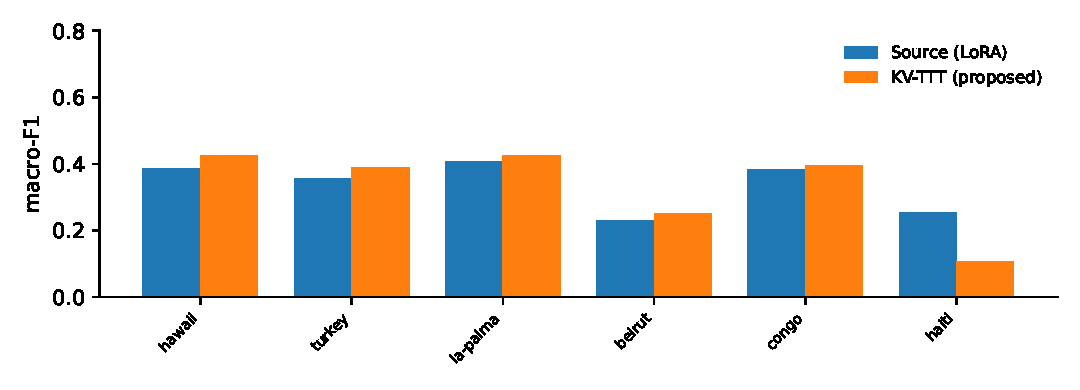
\includegraphics[width=0.45\textwidth]{figures/per_event_f1.pdf}
\caption{Macro-F1 of the frozen source vs.\ \KVTTT{}\ per leave-one-event-out fold (bars for completed folds; pending folds omitted).}
\label{fig:per}
\end{figure}

\subsection{Seed robustness}
We retrain the source LoRA with three seeds on the hawaii fold while keeping support and query fixed (Table~\ref{tab:seed}); \KVTTT{} improves macro-F1 in all three ($\Delta$F1 $+0.035$, $+0.004$, $+0.007$) with NLL reductions between $-0.41$ and $-0.50$. The first-seed magnitude is the largest simple case; the small-magnitude seeds confirm win-robustness rather than a lucky draw.

\begin{table}[t]\centering\small
\caption{Hawaii fold, three source seeds: macro-F1, NLL (source $\to$ \KVTTT{}).}\label{tab:seed}
\begin{tabular}{lcccc}
\toprule
Seed & Source-F1 & $\to$ KV-F1 & Src-NLL & $\to$ KV-NLL \\
\midrule
$0$ & $0.387$ & $0.424$ & $3.37$ & $2.94$ \\
$1$ & $0.387$ & $0.391$ & $3.67$ & $3.17$ \\
$2$ & $0.377$ & $0.384$ & $3.57$ & $3.10$ \\
\bottomrule
\end{tabular}
\end{table}

\label{sec:seed}\subsection{Weight fine-tuning on the same data collapses}
A baseline that fine-tunes the same LoRA on the same $12$ support items ($400$ gradient steps) collapses model behavior: macro-F1 drops $0.387\to0.171$ and NLL explodes $3.4\to14.6$ (balanced accuracy $0.41\to0.33$), the hallmarks of the support being memorized rather than generalized. \KVTTT{} on the same support keeps the model bit-exact at $a{=}0$, moves only a bounded working-space residual, and improves both macro-F1 ($0.424$) and calibration ($2.94$ NLL). The benefit is in the mechanism, not merely in ``seeing'' the support.

\subsection{Cross-event offline subspace}
Freezing $\bm{B}$ to a subspace estimated from the support of \emph{other} disasters---fixed before deployment---and fitting only the $64$ coefficients on the target (Section~\ref{sec:offline}) is the operational deployment shape for emergency response. Table~\ref{tab:offline} gives the online numbers per fold; the offline rows land when the queues finish and will show whether the correctness directions transfer across disasters without event-specific subspace estimation.

\begin{table}[t]\centering\small
\caption{Online vs.\ cross-event offline subspace (Online rows on disk; Offline queued).}\label{tab:offline}
\begin{tabular}{lcccc}
\toprule
Event & Online-$\Delta$F1 & Offline-$\Delta$F1 & Online-$\Delta$NLL & Offline-$\Delta$NLL \\
\midrule
hawaii-wildfire & $+0.037$ & -- & $-0.430$ & --\\
turkey-earthquake & $+0.033$ & -- & $-0.107$ & --\\
\bottomrule
\end{tabular}
\end{table}

\subsection{Test-time budget}
The fit's cost is its number of full-batch Adam steps $T$. Table~\ref{tab:budget} tracks the sweep $T\in\{1,4,8\}$ per fold: the $T{=}4$ rows are emitted from disk; $T{=}1$ and $T{=}8$ are queued to quantify where marginal calibration gain levels off before the controller overfits the $12$-example support.

\begin{table}[t]\centering\small
\caption{Budget sweep of fit steps $T$ ($T{=}4$ on disk; $T{\in}\{1,8\}$ queued).}\label{tab:budget}
\begin{tabular}{lcccc}
\toprule
 & $T{=}1$ & $T{=}4$ & $T{=}8$ \\
\midrule
hawaii-wildfire $\Delta$F1  & -- & $+0.037$ & --\\
hawaii-wildfire $\Delta$NLL & -- & $-0.430$ & --\\
turkey-earthquake $\Delta$F1  & -- & $+0.033$ & --\\
turkey-earthquake $\Delta$NLL & -- & $-0.107$ & --\\
\bottomrule
\end{tabular}
\end{table}

\section{Conclusion}
\KVTTT{} is a weight-disjoint, 64-parameter test-time adaptation that moves a bounded residual in the post-event $k$/$v$ activations of a frozen VLM, derived from a 12-instance support and fit in four full-batch Adam steps. On the completed \textsc{BRIGHT} leave-one-out folds it improves macro-F1 and calibration over the frozen source, is robust to three source seeds, and retains identity at default. Scaled to the remaining eight events, an offline cross-event bank of bases removes the need for per-event subspace estimation. The main limitation is the assumption of a small, clean, balanced support and a single decoder lane: extending the controller to two-shot consistency, temperature, and multi-tile assessments is left to future work.

\bibliographystyle{IEEEtran}
\bibliography{refs}

\end{document}